\chapter{Introducción}
\label{c:introduccion}
\vspace{1cm}
En este capítulo se presenta la motivación del desarrollo de este proyecto, seguido de una descripción del estado del arte del reconocimiento de objetos y algunas de sus aplicaciones en realidad aumentada. Tras ello, se exponen los objetivos generales y específicos de esta tesis, como así también los alcances de la misma.
\section{Motivación}
Las imágenes y videos presentes en el mundo digital, combinados con la potencialidad que ofrecen los ordenadores 
actuales, han hecho más fácil la creación de aplicaciones sofisticadas en el área de procesamiento de imágenes y visión computacional \cite{citeulike:9456628}.

Los seres humanos reconocemos fácilmente gran cantidad de objetos, independientemente del punto de vista en que se mire, las condiciones de iluminación, su tamaño, escala o incluso si se encuentran rotados, trasladados u obstruidos. Sin embargo, esta tarea no resulta trivial en el área de visión computacional. Así, el reconocimiento de objetos se puede resumir en el objetivo de buscar un objeto particular dado en una imagen o un video (secuencia de imágenes). 

La tarea de buscar puntos correspondientes entre dos imágenes de una misma escena u objeto es usada en una gran variedad de sistemas de visión computacional. La búsqueda de estos puntos, se realiza mediante detectores de puntos claves cuyo desafío es poder encontrar en una imagen puntos que sean fácilmente identificables y a la vez robustos a diferentes transformaciones. Así, estos detectores se convierten en la base de gran cantidad de herramientas basadas en visión computacional como ser el reconocimiento de objetos, vigilancia por video, imágenes médicas, la realidad aumentada y la restauración de imágenes entre otros.
%http://www.chrisevansdev.com/computer-vision-opensurf.html

Un sistema de realidad aumentada (RA) reemplaza parte del mundo real con objetos virtuales (generados por computadoras), los cuales parecen coexistir en el mismo espacio que el ambiente real cuando se lo ve a través de un dispositivo de visualización.
Si bien existen ampliaciones a esta definición, se puede definir a un sistema de realidad aumentada como aquel que posee las siguientes propiedades \cite{Azuma:2001:RAA:616073.618862}:
\begin{itemize}
 \item combina objetos virtuales y reales en un mismo ambiente,
 \item trabaja interactivamente y en tiempo real y
 \item detecta y realiza un ``seguimiento'' de objetos reales y virtuales entre sí.
\end{itemize}

Desde hace tiempo, los sistemas de realidad aumentada (del inglés, Augmented Reality) y reconocimiento de objetos,
han pasado a ser un tema pujante en el área de visión computacional, tomando gran 
interés en la comunidad científica y viéndose esto reflejado en diversidad de aplicaciones:
en el área del e-commerce - publicidad  \cite{5478308}, robótica \cite{conf/icra/2010}, juegos \cite{5711053,Azuma:2001:RAA:616073.618862}, libros interactivos \cite{KimPW09},
industria \cite{conf/visapp/BenhimaneNGGNM08}; en diferentes ambientes \cite{conf/ismar/KleinM07, Takacs:2008:OAR:1460096.1460165, conf/ismar/MiyashitaMTOESGGAL08}, aplicable sobre diferentes objetos 
\cite{conf/ismar/2007, Lepetit:2005:MMT:1166405.1166406, conf/iswc/2007} y llevada a cabo mediante el uso de distintos dispositivos \cite{WagnerRMDS10}.

La habilidad de reconocer e identificar objetos como imágenes, texto, logos, etc. en una imagen o video para luego ser usados como ``patrones'', es esencial en aplicaciones de RA, además de ser usada en control de calidad, vigilancia e identificación visual \cite{5739718}.
%y es por ello que en este trabajo nos centraremos en este tema.

Existe una distinción en RA entre dos tipos de sistemas \cite{1320421}: 
\begin{itemize}
 \item los que usan marcadores (\textbf{Marker based}), en los cuales se identifica un ``marcador artificial'' colocado en el ambiente, y por ende alterando el mismo y,
 \item los que no usan marcadores (\textbf{Markerless}), que se sustentan en usar características naturales para identificar objetos del mundo real, es decir, que no usan un ``marcador artificial'' para asistir al reconocimiento del objeto.
\end{itemize}
En ambos casos, el objeto 2D o 3D virtual da la apariencia de aparecer ``pegado'' al marcador o a la característica natural cuando se ve a través del área de visualización de RA.

De la misma forma para la detección y seguimiento de objetos, existen diferentes métodos \cite{1320421}, entre los cuales se pueden nombrar:
\begin{itemize}
 \item seguimiento basado en localización: involucra sensores como GPS, acelerómetros, giroscopios, etc. para identificar el objeto y su posición (por lo general menos precisos).
 \item seguimiento óptico: se basa en el análisis e identificación de características a partir de la imagen de forma tal que permitan identificar y obtener la posición del objeto.
 \item una combinación de los dos anteriores.
\end{itemize}

En este trabajo nos enmarcaremos en sistemas de RA sin marcadores y con detección y seguimiento de objetos que realicen un procesamiento de las características de la imagen, es decir, el método de seguimiento óptico.

Así, se propone construir un método con las características anteriormente nombradas, que permita reconocer objetos planos e identificar su posición en la imagen, en un ambiente controlado, para la posterior aplicación de realidad aumentada. 

El desarrollo de un motor propio de RA que sea fácilmente adaptable a aplicaciones específicas (comerciales, educativas, lúdicas, etc.) resulta de gran interés propio y para el grupo del \textit{SINC}, ya que si bien existen software similares desarrollados, no todos trabajan en tiempo real, otros son distribuidos bajo licencias privativas o utilizan marcadores artificiales, entre otras características que no lo hacen de interés para el grupo de trabajo. Además, se trabaja en una tecnología de punta que se encuentra en auge en estos tiempos y que presenta un futuro próspero. Una de las piezas fundamentales del motor citado, son los métodos de identificación y reconocimiento de objetos los cuales serán expuestos en el presente trabajo. Para ello, será necesario aplicar conocimientos de visión computacional \cite{citeulike:3484001, citeulike:9456628, bb1919} e investigar métodos de extracción de características en imágenes \cite{Nixon:2002:FEI}. Existe gran cantidad de investigaciones en el área, tales como:
\begin{itemize}
 \item el estudio de descriptores visuales \cite{BouGar} y locales \cite{bb53077, TuytelaarsM07, BenhimaneNGGNM08}, entre los cuales se encuentran el detector rápido de características robustas SURF (del inglés, Speeded-Up Robust Features) \cite{Bay:2008:SRF} y la transformación de características invariante a la escala SIFT (del inglés, Scale Invariante Feature Transform) \cite{bb48614}, etc.
 \item el reconocimiento de puntos claves \cite{bb36798},
 \item la detección en tiempo real de objetos \cite{conf/cvpr/HinterstoisserLIFN10},
 \item el seguimiento sin marcadores \cite{5607509},
 \item el análisis de características invariantes en imágenes \cite{conf/ismar/2004, Lowe:2004:DIF:993451.996342} y
 \item la clasificación de puntos característicos \cite{oai:infoscience.epfl.ch:52666}, entre otros.
\end{itemize}
Dichos temas, se tratan de abordar en menor o mayor medida para el correcto desarrollo del presente proyecto.
\section{Estado del arte}
% \section[Subtítulo corto]{Subtítulo largo}
% 
La realidad aumentada es una tecnología que utiliza la generación por computadora de objetos virtuales, para mezclarlos en una secuencia de imágenes reales. De modo diferente al concepto de Realidad Virtual, un sistema de RA permite al usuario ver el ambiente real con los objetos virtuales interactuando en él.
% La ``registración'' conocida como la estimación de la posición y el seguimiento de la cámara, es usada para obtener las variables del movimiento de la cámara ya sea mediante hardware o métodos de visión computacional o una combinación de ambos tanto en tiempo real como en aplicaciones off-line.
% 
% Los métodos de registración puede ser clasificados básicamente en 2 tipos:
% \begin{itemize}
%  \item basados en modelos (model based)
%  \item basados en movimiento y coincidencias (move-matching based).
% \end{itemize}

Cuando se tienen imágenes de una misma escena, las correspondencias 2D pueden ser extraídas en cada fotograma para estimar la posición del objeto buscado mediante la identificación de puntos característicos naturales (cuando se trata de RA sin marcadores) o marcadores artificiales que actúan como patrones alterando la naturalidad de la escena mediante una imagen artificial.
\subsection{Conceptos en realidad aumentada}
La RA permite enriquecer la perspectiva superponiendo objetos virtuales (2D o 3D) en el mundo real, con el objetivo de lograr persuadir al 
observador y dando la sensación de que el objeto virtual forma parte del ambiente real. De esta forma, se puede interpretar
la RA, como una mezcla entre un mundo real y uno virtual tal como se visualiza en el Diagrama continuo de Realidad-Virtualidad propuesto en \cite{Milgram94augmentedreality} y mostrado en la Fig. \ref{fig:Reality-Virtuality Continuum}.
\begin{figure}[tbp]
\centering
\scalebox{0.4}{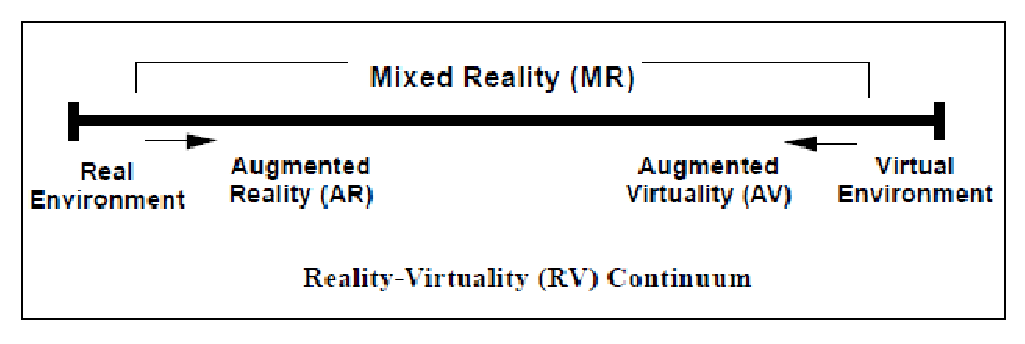
\includegraphics{../img_ent1/reality_virtual.eps}}
\caption[Diagrama continuo de Realidad-Virtualidad]{Diagrama continuo de Realidad-Virtualidad (Figura adaptada de \cite{Milgram94augmentedreality}).}
\label{fig:Reality-Virtuality Continuum}
\end{figure}

Algunos de los conceptos que se manejan en realidad aumentada son los siguientes:
\begin{description}
  \item [Vista real] 
  Se refiere a la secuencia o flujo de video producido por la cámara. La aplicación de RA captura imágenes desde esta secuencia de video, aumentándolas con objetos virtuales para crear una ``vista aumentada''. \cite{1320421}
  \item [Identificación y seguimiento (registration \& tracking)] 
  Describe los\\ métodos disponibles para alinear un objeto virtual con un sistema de coordenadas 
  en tres dimensiones en una vista real. En el seguimiento, se pueden distinguir entre diferentes métodos: \textit{seguimiento basado en localización} y \textit{seguimiento óptico} o una combinación de ambos \cite{conf/iswc/2007, 1320421}.
  %================
  %================
  \item[Punto de interés (POI)]
  Es un elemento de información asociado con una ubicación geográfica (longitud, latitud, altura) o un patrón visual (marcador, tapa de libro (sin marcadores), etc.) que se puede representar de alguna forma por la aplicación de RA \cite{1320421, Azuma:2001:RAA:616073.618862}.
  % El tipo de dato del punto de interés debe proporcionar una descripción de la localización o imagen de referencia utilizado en el seguimiento 
  % y el tipo de contenido que se dibujará (normalmente el contenido en si mismo (modelo 3d, imagen, etc) no es parte del 
  % punto de interés, pero un enlace al contenido se suministra en su lugar.
  %================
  %================
  \item [Objeto virtual] 
  Es algún tipo de contenido digital que es dibujado por la aplicación de RA y es superpuesto en la vista real. 
  Por lo general, incluye modelos 3D, imágenes 2D, iconos, textos, o incluso elementos no visuales como audio, entre otros \cite{conf/iswc/2007}, \cite{1320421}. 
  \item [RA basadas/no basadas en marcadores] 
  Cuando es utilizado el reconocimiento de imágenes para alinear un objeto virtual (seguimiento óptico), hay una distinción entre sistemas:
  los que identifican un \textit{marcador artificial} como un código matricial 2D colocado en un lugar determinado o sobre algún objeto del mundo real y los que utilizan la \textit{detección de características naturales de los objetos}, para identificar objetos del mundo real inalterados (como tapas de libros, posters, etc.), los cuales no poseen marcas artificiales que asistan en el reconocimiento del objeto.
  En ambos casos, el objeto virtual 2D o 3D, aparece ``pegado'' al marcador o característica natural cuando se ve a través de la ventana gráfica de RA \cite{conf/iswc/2007}, \cite{1320421}.
  \item [Reconocimiento basado en localización] 
  Se refiere al reconocimiento basado en información de geo-localización, obtenida a partir de dispositivos o sensores de localización presentes en el dispositivo de adquisición de imágenes. Mediante estos sensores, los dispositivos (por ejemplo: teléfonos celulares, tabletas digitales, etc.) pueden tener información de la posición del objeto a detectar, mostrando información relacionada mediante realidad aumentada.
  El término, es usado para hacer una distinción entre sistemas que usan sensores de localización, en contraste con los que hacen seguimiento óptico del objeto usando técnicas de reconocimiento de imagen. El reconocimiento basado en localización, %posee por lo general menos precisión que los métodos ópticos y 
es aplicado sobre todo en ambientes exteriores \cite{1320421, Azuma:2001:RAA:616073.618862}.
  \item [Seis grados de libertad (del inglés, Six Degrees of Freedom -6DoF)] 
  Se refiere a la capacidad del sistema de seguimiento para mantener la alineación de un objeto del mundo real en un espacio tridimensional. Esto es, la capacidad de moverse hacia delante/atrás, arriba/abajo, izquierda/derecha (traslación en tres ejes perpendiculares), combinados con la rotación sobre tres ejes perpendiculares.

  La reconstrucción de la posición de la cámara con 6DoF es el objetivo más importante en RA, ya que de esta manera se determina la posición de la cámara y, en consecuencia se obtiene la posibilidad de poder dibujar los objetos virtuales en una perspectiva correcta \cite{conf/iswc/2007, 1320421, Azuma:2001:RAA:616073.618862}.
\end{description}
% \bigskip
% \textbf{Referencias de la sección:
% \cite{Milgram94augmentedreality}, %Paul Milgram et al., 1994 
% \cite{1320421}, %Ben Butchart, 2011
% \cite{conf/iswc/2007}, %Taehee Lee et al., 2007 6dof
% \cite{Azuma:2001:RAA:616073.618862}, %Ronald Azuma et al., 2001
% \cite{5739718}.% Ahyun Lee et al., 2010  sift lkt
% }
\subsection{Puntos característicos y descriptores}
\label{sec:ptos_caract_descriptores}
La detección de puntos característicos y los descriptores de imágenes, son una característica ampliamente usada en problemas de reconocimiento de objetos, detección de imágenes, seguimiento visual, reconstrucción 3D entre otras aplicaciones. El objetivo es seleccionar ciertos puntos claves en una imagen, de forma que estos permitan distinguirla de otras sin la necesidad de tener que analizar la totalidad de la imagen.
Esta aproximación funciona correctamente en la medida que se detecten la cantidad suficiente de puntos de interés que sean ``distinguibles'' y, a su vez, estables para que puedan ser nuevamente localizados en otra escena.

\subsubsection{Características locales}
\label{c:deteccioncaracteristicas}
Una característica local puede ser interpretada como un patrón de imagen que difiere de su vecindad y puede venir representada por ejemplo por un punto, un borde o pequeños trozos de la imagen. Es común la realización de ciertos cálculos sobre una región alrededor de la característica local detectada y su resultado se convierte en un vector numérico el cual recibe el nombre de descriptor. Estos últimos pueden ser utilizados para gran variedad de aplicaciones.

Se puede hacer una distinción de los detectores de características, dependiendo del uso que se le de a los mismos:
\begin{itemize}
 \item \textit{Características locales específicas que otorgan una interpretación semántica de un contexto limitado específico}, por ejemplo: de bordes detectados en imágenes aéreas, se puede decir que comúnmente corresponden a caminos o rutas.
 \item \textit{Características locales que proveen un conjunto limitado de puntos bien localizados e individualmente identificables}. En este caso, lo que representa la característica no es realmente relevante. Lo importante es que su ubicación pueda ser determinada con exactitud y de manera estable en el tiempo, por ejemplo situaciones de correspondencia de puntos y seguimiento de los mismos, calibración de la cámara y reconstrucción 3D.
%  \item \textit{Características locales que pueden ser usadas como una representación robusta de la imagen permitiendo reconocer objetos o escenas sin la necesidad de segmentación}. Aquí no es relevante lo que la característica represente, ni tampoco es necesario que pueda ser precisamente localizada, sino que lo que importa es un análisis del tipo estadístico. Aplicaciones como la clasificación de escenas y análisis de texturas se encuentran dentro de esta categorización.
\end{itemize}

Los dos escenarios aquí planteados no resultan ser los únicos posibles, pero se exponen con el objetivo de enfatizar las diferentes propiedades requeridas para diversas situaciones. Claramente cada uno de los escenarios, impone restricciones sobre los puntos característicos a utilizar. En este trabajo, nos enfocaremos particularmente en el segundo caso (correspondencia de puntos y estabilidad de los mismos).
% \subsection{Características locales y globales}
% 
% La importancia de las características locales ha sido demostrada en el contexto de reconocimiento de objetos por el sistema visual humano \ref{Biederman87recognition-by-components:a}. Los experimentos, han demostrado que la eliminación de esquinas en las imágenes impiden el reconocimiento humano, mientras que si se quita la mayor parte de la información de bordes rectos, la imagen aún resulta identificable. Un ejemplo de esto puede ser apreciado en la figura \ref{fig:lineandedgesimportance}.
% 
% \begin{figure}[tbhp]
%    \centering
%         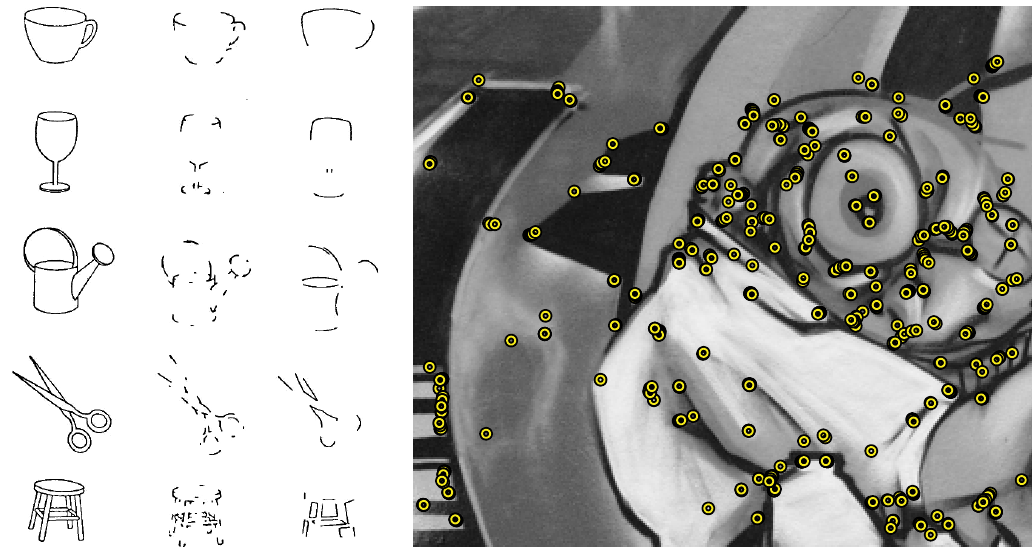
\includegraphics[scale=0.4]{figs/lineandedgesimportance}
%     \caption[Respuestas del descriptor SURF]{Izquierda: Importancia de las esquinas y uniones en reconocimiento visual \ref{Biederman87recognition-by-components:a}. Derecha: Puntos de interés extraídos por un detector de esquinas/bordes. Imagen tomada de \ref{Tuytelaars:2008:LIF:1481563}}
%    \label{fig:lineandedgesimportance}                %% Etiqueta para la figura entera
% \end{figure}
\subsubsection{Propiedades de características locales}
Las características locales comúnmente vienen representadas por una extensión espacial, por ejemplo una vecindad de píxeles de un punto de interés dado. Los detectores seleccionan características locales basadas en la intensidad de los patrones subyacentes.

Las características son consideradas útiles cuando poseen las siguientes propiedades:
\begin{itemize}
 \item \textbf{Repetibilidad}: dadas dos imágenes tomadas bajo diferentes condiciones del mismo objeto o escena, un alto porcentaje de las características detectadas debe poder ser encontrada en ambas imágenes.
 \item \textbf{Distintividad}: los patrones de intensidad subyacentes a las características detectadas deberían mostrar variaciones significativas, de forma tal que las características sean distinguibles y se puedan encontrar posteriormente pares de correspondencias.
 \item \textbf{Localidad}: Las características deberían ser locales (en el sentido de tener una extensión espacial acotada) para reducir la posibilidad de oclusión y permitir un modelo de aproximación a las deformaciones geométricas y fotométricas entre dos imágenes tomadas bajo diferentes condiciones visuales. %(por ejemplo, basadas en la hipótesis de asumir que a nivel local son planas)(por ejemplo, basadas en la hipótesis de planaridad local). CUALES SON???
 \item \textbf{Cantidad}: El número de características detectadas debe ser lo suficientemente grande para que aún en objetos pequeños, una cantidad razonable de éstos puedan ser detectada. Esta cantidad depende de la aplicación y, por lo general, puede ser adaptada mediante un umbral. La densidad de las características debe reflejar el contenido de información de la imagen de forma de proveer una representación compacta de la misma.
 \item \textbf{Precisión}: Las características detectadas deberían ser precisamente localizadas respecto a la posición en la imagen, al tamaño de la misma y en lo posible a su forma.
 \item \textbf{Eficiencia}: la detección de características en una imagen nueva, debería poseer tiempos lo más acotados posibles para una aplicación.
\end{itemize}

La Repetibilidad es comúnmente una de las propiedades de mayor importancia y se puede lograr alcanzando dos propiedades, invariancia y robustez:
\begin{itemize}
 \item \textbf{Invariancia}: si se esperan grandes deformaciones, la idea consiste en modelar matemáticamente las mismas de forma de tener un método de detección de características que no se vea afectado por dichas transformaciones matemáticas.
 \item \textbf{Robustez}: en el caso de deformaciones relativamente pequeñas, por lo general es suficiente con hacer que los métodos de detección de características resulten menos sensitivos a dichas deformaciones, por ejemplo, la precisión de la detección puede decrecer pero no debería hacerlo de forma drástica. Algunas deformaciones típicas que se pueden afrontar mediante la robustez son: el ruido en la imagen, los efectos de discretización, el borroneado, como así también las desviaciones geométricas y fotométricas del modelo matemático utilizado para obtener invariancia.
\end{itemize}

La importancia de las propiedades mencionadas, dependen de la aplicación sobre la cual se trabajará. El ajuste de éstas, conlleva un compromiso y se fortalecerán unas u otras dependiendo de cada caso en particular.

La \textit{localización} y \textit{distintividad} son propiedades interdependientes que no pueden ser maximizadas simultáneamente: cuanto más local es una característica, menos información está disponible sobre el patrón de intensidad subyacente y se hace más difícil de encontrar la correspondencia correcta (distintividad). Por otro lado, en el caso de objetos planos o rotación de cámaras, las imágenes están relacionadas por la homografía global, y no existen problemas con las oclusiones o discontinuidad de profundidades. Bajo estas condiciones, la cantidad de características locales puede ser incrementada sin problemas, resultando ser altamente distintivas, pero impactando negativamente en la \textit{eficiencia}.

Similarmente, al incrementar el nivel de \textit{invariancia}, se reduce la \textit{distintividad}. Un análisis similar se puede hacer entre \textit{robustez} y \textit{distintividad}, típicamente cierta información (considerada ruido) es descartada con el objetivo de lograr \textit{robustez}. Como resultado, es importante tener una idea clara del grado requerido de invariancia o robustez para una aplicación específica. Es difícil alcanzar alta invariancia y robustez al mismo tiempo.

La \textit{precisión} es especialmente importante cuando se precisan usar correspondencias, por ejemplo, para estimar la geometría epipolar o calibrar una cámara.

La \textit{cantidad} es particularmente útil en métodos de reconocimiento de objetos o escenas, donde es importante cubrir densamente el objeto de interés. Sin embargo y como se ha mencionado, una gran cantidad de características impacta negativamente en el tiempo de computo.
\subsection{Detección y correspondencia de puntos de interés}
En visión computacional, el concepto de puntos de interés (puntos claves) o puntos característicos, como la correspondencia entre los mismos resultan ampliamente usados en diversas tareas. La idea consiste en seleccionar algunos puntos especiales de la imagen (una cantidad suficiente) que sean distinguibles, estables, posean repetibilidad y puedan localizarse como se describió en la Sec. \ref{c:deteccioncaracteristicas}.

La búsqueda de correspondencia de puntos discretos en imágenes, puede ser dividida en tres grandes pasos:
\begin{itemize}
 \item Primeramente, los puntos de interés (esquinas, uniones de tipo T, etc.) son seleccionados como características distintivas de la imagen. La propiedad más sobresaliente de un detector de puntos de interés es su repetibilidad que expresa la robustez del detector en buscar los mismos puntos de interés bajo diferentes condiciones de visualización.
 \item Luego, se representa la vecindad de cada punto de interés detectado mediante un vector de características (vector descriptor). Idealmente, este descriptor debe ser distintivo, robusto al ruido, a la detección de desplazamientos y a las deformaciones geométricas o fotométricas de la imagen.
 \item Finalmente, se buscan las correspondencias entre los vectores descriptores de las imágenes. Dicha correspondencia, generalmente se encuentra basada en la distancia entre los vectores (por ejemplo: la euclídea). La dimensión del descriptor impacta directamente en el tiempo de cálculo. Así, buscar correspondencias entre vectores de bajas dimensiones resulta más rápido, pero a su vez los vectores se hacen menos distintivos. Como contraparte vectores de altas dimensiones involucran altos tiempos de procesamiento logrando mayor distintividad.
\end{itemize}

% Es nuestro objetivo seleccionar un detector y descriptor que cumpla los requisitos mínimos para la realización de este trabajo.
Cuando se trabaja con características locales uno de los primeros inconvenientes a resolver es obtener un alto nivel de invarianza. Claramente, esto depende de las deformaciones geométricas y fotométricas que pueda sufrir la imagen. En nuestro caso, nos centraremos en los cambios de escala y la rotación en el plano, asumiendo que los efectos de segundo orden: inclinación, perspectiva y anisotropía son cubiertos en cierto grado por la robustez global del descriptor utilizado. En cuanto a las deformaciones fotométricas, se asume un modelo lineal simple con un desplazamiento y un cambio de contraste (factor de escala).

En este trabajo, se tratará con características locales, las mismas describen una parte de la imagen; en contraposición con las características globales que describen la imagen como un todo.

Existen diferentes tipos de características locales: aquellas que se basan en líneas o curvas (detectadas por ejemplo con la transformada de Hough \cite{Duda:1972:UHT:361237.361242}) y otras como las que utilizaremos en este trabajo que se valen de puntos característicos, como esquinas, bordes, etc.
% Existe gran variedad de algoritmos de detección de puntos claves y características. 
% \item el detector ``Buenas características a seguir'' (Good Features to track) \ref{Shi_1994_3266}, cual esta basado en los eigen valores de la Matriz Hessiana para determinar si un punto es una esquina.
%  \item Regiones extremas mas estables (Most Stable Extremal Regions o MSER) \ref{DBLP:journals/ivc/MatasCUP04},que identifica regiones de una imagen cuyos píxeles son más brillantes u oscuros que los píxeles vecinos. %con rendimiento de $\mathcal{O}(n)$ basado en la cantidad de píxeles
%  \item Características por test de segmento acelerado (Features From Accelerated Segment Test o FAST) \ref{Rosten05fusingpoints, citeulike:9456628} que compara los valores de los píxeles en un circulo alrededor del punto y se fija en los arcos continuos que son más oscuros o más claros que el punto en si mediante un umbral determinando de esta forma una esquina. Este algoritmo se caracteriza por ser rápido comparado con otros detectores (como el detector de Harris), mientras mantiene un grado de repetitibilidad similar.
Por ejemplo, para obtener esquinas, uno de los más usados es el detector de esquinas de Harris \cite{Harris88acombined, citeulike:3484001}, el cual está basado en los eigenvalores de la matriz de segundo orden para determinarlas, aunque no resulta invariante a escala. Otros detectores de características como el detector de regiones extremas más estables %o MSER 
\cite{DBLP:journals/ivc/MatasCUP04} y el de características por test de segmento acelerado %o FAST 
\cite{Rosten05fusingpoints, citeulike:9456628} se encuentra también en gran parte de la bibliografía.

El concepto de selección de escala automática \cite{springerlink:10.1023/A:1008045108935} permitió detectar puntos asignándole una escala (tema que será tratado en la Sec. \ref{sec:invarianza_a_escala}) a cada uno de ellos. Para la detección de los mismos, se experimentó tanto con el determinante de la matriz hessiana como con el laplaciano (traza de la matriz hessiana). Otros autores \cite{conf/iccv/MikolajczykS01} refinaron este método, creando un detector de características robusto e invariante a escala, logrando una alta repetibilidad. De esta manera, surgió el detector \textit{Harris-Laplace} y \textit{Hessian-Laplace}. Para el primero de ellos, se utiliza una medida de harris para seleccionar la ubicación de la característica y el laplaciano para seleccionar la escala. Para el caso del detector \textit{Hessian-Laplace} se utiliza el determinante de la matriz hessiana para seleccionar la ubicación de la característica y el laplaciano para seleccionar la escala.

Enfocado en la velocidad, Lowe \cite{Lowe1999} propuso aproximar el laplaciano del gaussiano (LoG) mediante filtros diferencia de gaussianos (DoG). Otros detectores de puntos de interés invariantes a escala fueron propuestos, el detector de regiones salientes \cite{journals/ijcv/KadirB01} que utiliza la maximización de la entropía en la región y el detector de regiones basado en bordes \cite{conf/cvpr/JurieS04} que detecta regiones locales convexas sobre contornos de imagen, entre otros.

Del estudio de los detectores existentes y de las comparaciones en diferentes publicaciones \cite{journals/ijcv/MikolajczykS04, bb53077}, se ha concluido que los detectores basados en el hessiano son los más estables y poseen mayor repetibilidad que los basados en esquinas de harris. Incluso, se han obtenido mejores resultados mediante el uso del determinante de la matriz hessiana en lugar de la traza de la misma \cite{journals/ijcv/MikolajczykS04}. También, se ha observado que las aproximaciones como el DoG pueden aumentar la velocidad a un bajo costo en términos de precisión. Así, surgió SIFT \cite{Lowe:2004:DIF:993451.996342} que calcula un histograma de los gradientes orientados localmente alrededor del punto de interés y genera un vector característico de 128-dimensiones. Luego, se propusieron varios refinamientos a este esquema básico como el análisis de componentes principales - transformación de características invariante a la escala (PCA-SIFT: del inglés, Principal Components Analysis - Scale Invariant Feature Transform) \cite{citeulike:3484001}, \cite{bb53077} que construye un descriptor de 36 dimensiones. De esta forma es más rápido el proceso de buscar coincidencias, aunque pierde distintividad y velocidad en el cálculo de características respecto a SIFT \cite{Mikolajczyk:2005:PEL:1083822.1083989}. De esta manera, el método SIFT se consolidó como el más adecuado para usos prácticos, resultando distintivo y relativamente rápido lo cual resulta crucial en aplicaciones ``on-line''.

Más tarde y basados en las ideas de SIFT, se propuso un nuevo detector y descriptor de características denominado SURF \cite{Bay06surf:speeded, Bay:2008:SRF}. El mismo, se basa en ideas del SIFT e introduce algunas modificaciones respecto al uso de imágenes integrales, filtros caja y un método de indexación rápida para búsqueda de correspondencias, que permite generar un descriptor de 64 dimensiones que se calcula y compara más rápidamente, manteniendo una precisión y distintividad valorable.
\subsection{Búsqueda de correspondencias}
Existe una extensa variedad de publicaciones \cite{muja_flann_2009, AryaEtAl98, Beis:1997:SIU:794189.794431, Liu04aninvestigation} que abordan la búsqueda de correspondencias mediante el algoritmo de búsqueda del vecino más cercano, en los que su rendimiento varía dependiendo de las propiedades del conjunto de datos, tales como: la dimensionalidad, correlación, características de agrupación y tamaño. 
Uno de los algoritmos utilizados es KD-tree \cite{Beis:1997:SIU:794189.794431, Friedman:1977:AFB:355744.355745} (básicamente se trata de un árbol binario balanceado de búsqueda), el cual ha dado buenos resultados para la búsqueda exacta en datos de bajas dimensiones. Este algoritmo, ha sido modificado en diversos trabajos \cite{bb23918, AryaEtAl98, Beis:1997:SIU:794189.794431, VLDB95574, Fukunaga75, bb78856, bb79759, Liu04aninvestigation, bb77826} para lograr reducir los tiempos de ejecución con datos de grandes dimensiones, a coste de obtener resultados aproximados. En el trabajo de Slipa-Anan y Hartley \cite{Silpa_KDTree, bb77826}, se propuso el uso de múltiples árboles KD aleatorios conocidos por su término en inglés como \textbf{Randomized KD-Tree}, que obtiene resultados satisfactorios en un amplio rango de problemas \cite{muja_flann_2009} reduciendo los tiempos de cálculo.
\subsection{Transformación proyectiva}
Las imágenes son producidas usando una cámara, que captura la escena mediante la proyección de luz que pasa por la lente e impacta en un sensor. El hecho de que una imagen se forma a través de la proyección de una escena 3D en un plano 2D, impone la existencia de una importante relación entre la escena, la imagen y diferentes imágenes de la misma escena. La geometría proyectiva es la herramienta usada para describir y caracterizar, en términos matemáticos, el proceso de formación de la imagen.

Algunos de los conceptos fundamentales en esta temática involucran temas como: el modelo pin-hole de la cámara \cite{citeulike:3484001, citeulike:9456628}, la calibración de la cámara que arroja como resultado los parámetros de distorsión y la matriz que la caracteriza \cite{citeulike:3484001, citeulike:9456628, Azuma:2001:RAA:616073.618862}, la correspondencia de imágenes \cite{citeulike:3484001, citeulike:9456628}, el cómputo de la homografía para estimar la posición del objeto \cite{citeulike:3484001, citeulike:9456628, conf/icra/2010}, entre otros.
%%%%%%%%%%%%%%%%%%%%%%%%%%%%%%%%%%%%%%%%%%%%%%%%%%%%%%%%%%%%%%%%%%%%%%%%%%%%%%%%%%%%%%%%%%%%%%%%%%%%%
\section{Objetivos del Proyecto Final}
Una vez introducida la tarea de interés y el marco general de trabajo, se enuncian a continuación los objetivos generales y particulares del presente Proyecto Final.
\subsection{Objetivos generales}
  \begin{itemize}
      \item Desarrollar un método para reconocer y seguir objetos en una secuencia de video digital y desarrollar un prototipo que haga uso del mismo aplicándolo a realidad aumentada.
      \item Afianzar y extender los conocimientos adquiridos en el cursado de la carrera Ingeniería en Informática.
  \end{itemize}
\subsection{Objetivos específicos}% poner objetivos medibles
\begin{itemize}
	\item Realizar el relevamiento del estado del arte en métodos utilizados para la detección y seguimiento de objetos en el Procesamiento Digital de imágenes.
	\item Diseñar y desarrollar un método reconocedor y seguidor de objetos planos en el flujo de video tomado por una cámara web estándar, sobre un ambiente controlado.
	\item Implementar el método en un algoritmo computacional que pueda ser utilizado en diferentes sistemas operativos.
	%\item Optimizar el procesamiento llevado a cabo para lograr método desarrollado para que sea aplicable en tiempo real (\textbf{procesamiento}). 
	\item Optimizar el procesamiento llevado a cabo para aplicarlo en tiempo real. 
	\item Implementar una aplicación prototipo específica (en el área de turismo, educación, publicidad, juegos u otros) aplicando el método desarrollado.
\end{itemize}
\section{Alcances del Proyecto Final}
En este proyecto se presenta un método para la detección de objetos planos en la escena y determinando su ubicación se superpone un objeto virtual para lograr ``enriquecer la realidad''.

Entre los alcances del proyecto se pueden enumerar los siguientes:
\begin{itemize}
  \item El trabajo se enmarcará en un sistema del tipo sin marcadores con método de reconocimiento del tipo seguimiento óptico.
  \item El proyecto involucra el desarrollo de un prototipo para ser utilizado en una computadora con una cámara web estándar. Cabe aclarar, que no se pretende realizar una aplicación final específica y completa (estudio y diseño de interfaz amigable al usuario, introducción amigable de parámetros, etc.) orientada al uso de un usuario final.
  \item Aunque no es un objetivo la implementación de varios métodos y su comparación, en una etapa previa se revisarán las características de algunos métodos para poder seleccionar alguno que se adecue a los requerimientos.
\end{itemize}